\chapter{Practical Design Guidelines of BOS Setups}
\label{chapter: methodology}

This chapter describes the methodology used to design the experimental setups. First, a brief description of the geometry of two optical setups is presented, one typical to BOS and another exclusive to SBOS. The standard BOS setup, discussed in subsection \ref{subsection: standard BOS geometry}, places the in-focus plane on the background reference behind the refractive object, as the conventional configuration described in the literature. Subsection \ref{subsection: Negative defocus geometry} then introduces the negative defocus setup, a configuration made possible only by SBOS, where the in-focus plane is positioned in front of the test subject. For both geometries, the governing equations relate performance parameters such as sensitivity, spatial resolution and speckle size to physical setup variables.

A design strategy was then envisioned to define the setup variables and explore how they interact across the feasible design space. Rather than solving the system for a single configuration, a MATLAB script was developed to compute the full set of variables X = ($S, s_{min}, \Delta s, d_f, Z, M, CoC, m$) for a range of combinations of the parameters P = ($f_\#, l, f$). This design space exploration, presented in section \ref{section: Design Strategy}, allows the main trends that govern the optical setup to be visualized through surface maps and provides insight into how focal length, defocus distance and f-stop number affect the trade-off between sensitivity and spatial resolution. The strategy is applied first to the SBOS configuration (subsection \ref{subsection: Surface Maps for SBOS}), then to the standard BOS configuration (subsection \ref{subsection: Surface maps for BOS}) for comparison, before the effect of the object field of view is examined in subsection \ref{subsection: Effets of FoV}. Section \ref{section: Summary of Practical Guidelines} then collects the outcomes of this exploration into a single set of practical design guidelines. Together, these sections establish the reasoning behind the final design choices used in the experimental setups described in Chapter \ref{chapter: Experimental Setups}.

\section{Geometries of a SBOS optical setup}
\label{section: Geometries of a SBOS optical setup}
Laser speckled background oriented schlieren opens the possibility of novel and unusual optical configurations that would be otherwise unfeasible for a standard BOS setup. A description of the geometry of a normal BOS configuration is given below, followed by the detailing of the negative defocus position. This section presents and compares the equations used for both setups. These formulas will be used to assess the difference in performance of a standard BOS setup and an exclusive SBOS configuration.

\subsection{Positive defocus setup}
\label{subsection: standard BOS geometry}
\par A positive defocus setup is the standard BOS configuration, where the in-focus plane is on the background reference behind the refractive object, as shown in Figure \ref{fig: Geometry BOS}. The Figure displays relevant distances for the design of the setup: $d_f$ corresponds to the distance of the in-focus plane to the camera lens, $m$ is the distance between the lens and the refractive object and $l$ is the distance between the test section and the in-focus plane, also called defocus distance. $Z$ is the distance between the lens and the formed image, following the ideal lens relationship. The latter is important if a single converging lens is used to collect light, however it is not so relevant when compound lenses such as the ones present on modern cameras are used. Other parameters to be defined are: the magnification $M$ of the object in the image plane, the lens focal length $f$ and the camera f-stop number $f_\#$. All these variables will be defined by the equations below.

\begin{figure}[htbp]
    \centering
    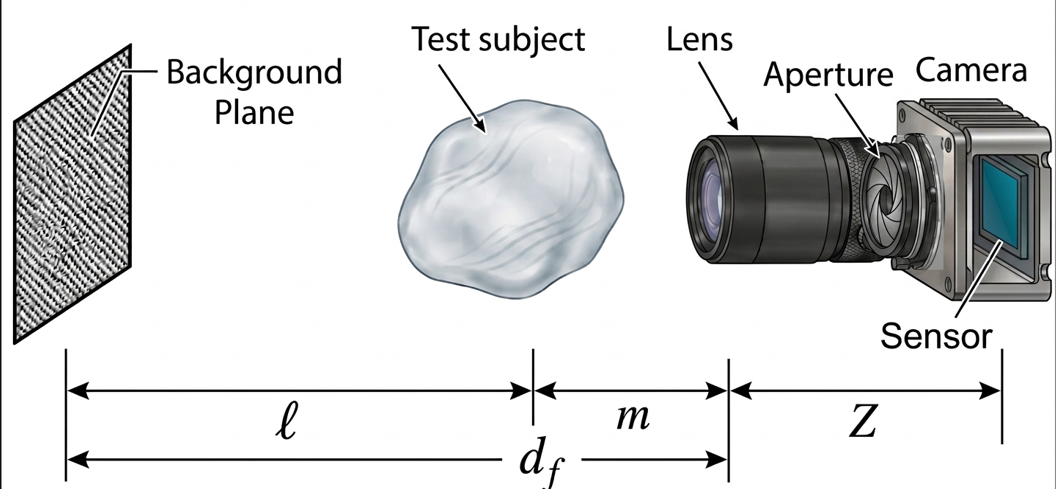
\includegraphics[width=0.6\textwidth]{figures/BOS setup.png}
    \caption{Geometry of a standard BOS Setup (positive defocus) }
    \label{fig: Geometry BOS}
\end{figure}

\par Equation \ref{equation: df} derives directly from Figure \ref{fig: Geometry BOS} and relates the distances $m, d_f$ and $l$. The defocus distance $l$ is measured from the refractive object to the in-focus plane, so it is treated as positive when the in-focus plane lies behind the object, and negative when it lies in front of it. The same equation therefore describes both geometries, with only the sign of $l$ changing.

\begin{equation}
    \label{equation: df}
    d_f = m + l
\end{equation}

\par For a first preliminary sizing, let's consider the camera lens as ideal. This permits the use of the gaussian thin lens equation (equation \ref{equation: Thin Lens equation}) and the coupled definition of magnification (equation \ref{equation: M}). In these equations, the object positioned at a distance $d_f$ from the lens is in focus and has its image at a distance $Z$ behind the lens with a magnification $M$. This formula comes with a specific convention regarding the sign of $M$, where negative $M$ corresponds to an inverted image and a positive to an upright image. Since a camera is being used, only the inverted image is going to be considered and for the sake of convenience this will be taken as positive. The camera also implies that $d_f > f$, as no image can form on the imaging sensor otherwise.

\begin{equation}
    \label{equation: Thin Lens equation}
    \frac{1}{f} = \frac{1}{d_f} + \frac{1}{Z}
\end{equation}

\begin{equation}
    \label{equation: M}
    M = \frac{Z}{d_f}
\end{equation}

As discussed in chapter \ref{chapter: LiteratureReview} Schwarz et al. \cite{Schwarz&Braukmann} and Gojani et al. \cite{Gojani&Obayashi} have drawn guidelines for the practical design of a BOS optical setup highlighting the importance of the sensitivity and spatial resolution. Sensitivity $S$ can be written as shown in equation \ref{equation: S BOS}, while the minimum distinguishable feature $s_{min}$ defined by Schwarz et al. \cite{Schwarz&Braukmann} is given by equations \ref{equation: CoC BOS} and \ref{equation: smin}.
%while the spatial resolution $s_{min}$ defined by Gojani et al. is written by equations \ref{equation: CoC BOS} and \ref{equation: d_av BOS} .

\begin{equation}
    \label{equation: S BOS}
    S = \frac{\Delta y}{\epsilon} = lM 
\end{equation}

\begin{equation}
    \label{equation: CoC BOS}
    CoC = \frac{lfM}{f_\#m}
\end{equation}

\begin{equation}
    \label{equation: smin}
    s_{min} = \frac{CoC}{2 \cdot M_{obj}}
\end{equation}

%\begin{equation}
%\label{equation: d_av BOS}
%    s_{min} = \frac{lM}{f_\#(M+1)} + \frac{CoC}{M} \left( 1 - \frac{l}{d_f}\right)
%\end{equation}
\par In equation \ref{equation: smin}, $M_{obj}$ is the blurred object magnification, which is defined by equation \ref{equation: M obj}.

\begin{equation}
    \label{equation: M obj}
    M_{obj} = \frac{L_{sens}}{L_{FoV_{obj}}}
\end{equation}

Equation \ref{equation: M obj} relates the field of view of the object and the camera sensor dimension. In the literature \cite{Schmidt2025, Schwarz&Braukmann}, many authors define the focal length $f$ by choosing a desired field of view of the object. They utilize equation \ref{equation: LFoVobj simplified} which is derived through the ideal lens equation and the definition of magnification. Thus it makes the fundamental assumption that the object is in focus as the ideal lens equation only applies to in-focus objects. Since the refractive object is out of focus, the assumption is fundamentally wrong and another equation must be derived to connect the lens' focal length to the blurred object's dimension. Geometry can be used to derive equation \ref{equation: LFoVobj BOS} without relying on the ideal lens relationship, the derivation can be found on Appendix \ref{Appendix: Blurred Object}.

\begin{equation}
    \label{equation: LFoVobj simplified}
    f = \frac{L_{sens}m}{L_{FoV_{obj}}+L_{sens}}
\end{equation}

%\par If the field of view of the object is small, blur plays a bigger role. The refractive object size differs from the one obtained before, which risks setting up a field of view that is too small than the one desired, consequently, losing information. In order to compute the $L_{FoV_{obj}}$ for small field of views, the same rationale used by Gojani et al. \cite{Gojani&Obayashi} can be used to derive equation \ref{equation: LFoVobj BOS}. Using this method, the test subject dimension is defined through the expanded cone of light that reaches the sensor screen. This way, the field of view of the captured object is more accurately estimated as it considers all the light that comes from the test section and reaches the sensor. The derivation of this equation can be found in the appendix.

\begin{equation}
    \label{equation: LFoVobj BOS}
    L_{FoV_{obj}} = \frac{m \cdot L_{sens}}{f(M+1)}
\end{equation}

%\par Since this project will test the standard BOS setup using laser speckles, the last equation is the Rayleigh diffraction limit, which is used to estimate the minimum speckle size $\Delta s$ \cite{Barker&Fourney}.

\subsection{Negative defocus setup}
\label{subsection: Negative defocus geometry}
Figure \ref{fig: SBOS with negative l} describes the geometry of a SBOS setting with negative defocus distance, which means that the in-focus plane is in front of the test subject. All the equations from the previous section remain valid in this case, that is, equations \ref{equation: df}, \ref{equation: Thin Lens equation}, \ref{equation: M}, \ref{equation: S BOS}, \ref{equation: CoC BOS}, \ref{equation: smin} and \ref{equation: LFoVobj BOS}. The single difference is that $l$ is now negative, so that equation \ref{equation: df} places the in-focus plane in front of the refractive object, as shown in Figure \ref{fig: SBOS with negative l}.
 
\begin{figure}[htbp]
    \centering
    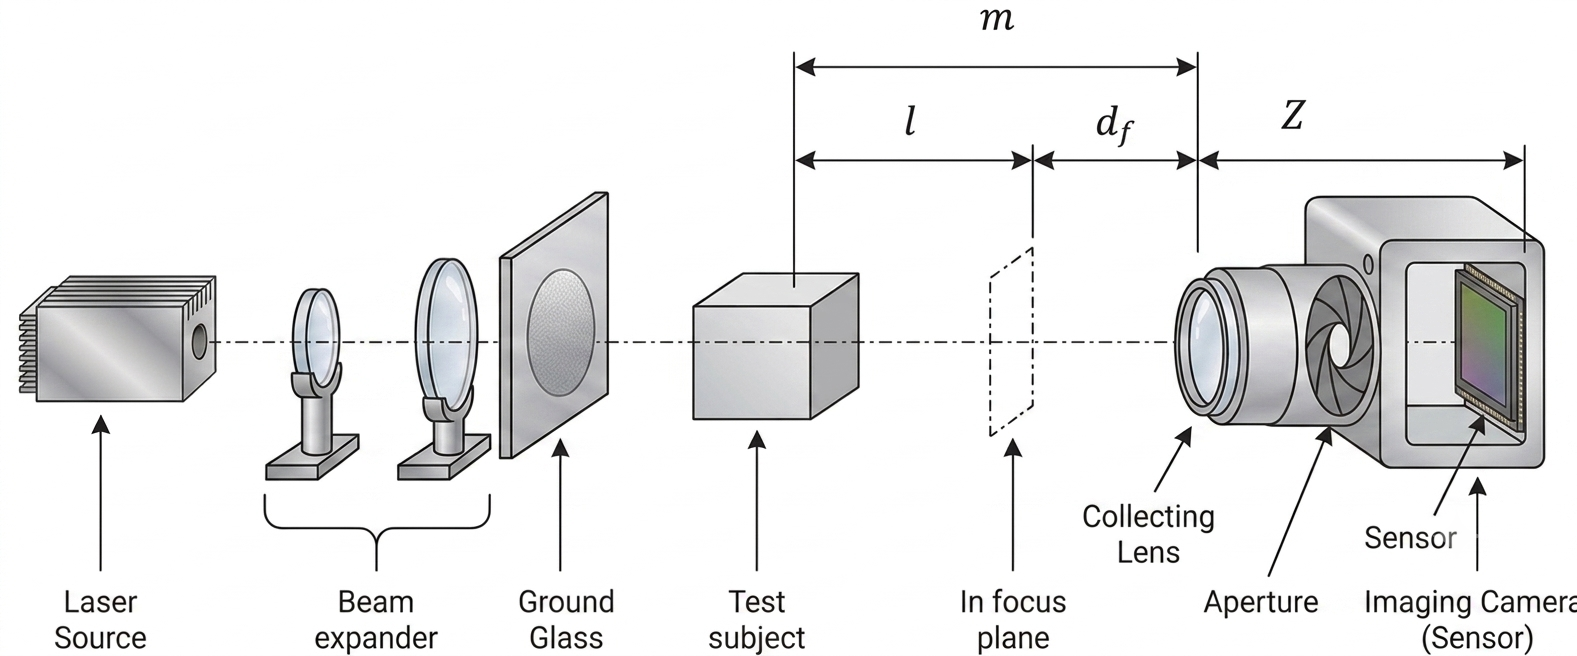
\includegraphics[width=0.6\textwidth]{figures/SBOS with negative l.png}
    \caption{Geometry of a SBOS setup with in-focus plane before the test subject (negative defocus) }
    \label{fig: SBOS with negative l}
\end{figure}

\par Another difference from BOS to SBOS is the speckle generation. Barker and Fourney \cite{Barker&Fourney} have used the Rayleigh limit to quantify the minimum speckle size when working with laser interferometry, the equation is presented as equation \ref{equation: Rayleigh Limit}.

\begin{equation}
   \label{equation: Rayleigh Limit}
   \Delta s = 1.22 \lambda f_\#(1+M)
\end{equation}


\par It has been mentioned in chapter \ref{chapter: LiteratureReview} that this configuration provides a better sensitivity for the same spatial resolution than standard BOS, this might be explained through a careful analysis of the setup geometry and the equations that govern it. In equation \ref{equation: S BOS}, $S$ is directly proportional to $M$, while in equation \ref{equation: M}, $M$ is inversely proportional to $d_f$. Comparing Figure \ref{fig: Geometry BOS} and Figure \ref{fig: SBOS with negative l}, it is clear that for the same defocus distance, $d_f$ is smaller in the latter case. Consequently, $M$ is larger and the sensitivity is higher. However, since $CoC$ also depends on $M$, it is not immediately obvious whether the gain in sensitivity is offset by the additional blur.
\section{Sensitivity-Resolution Ratio}
\label{section: Sensitivity-Resolution Ratio}
The dilemma of increasing sensitivity through magnification but also increasing blur can be solved by relating sensitivity and spatial resolution directly. Using the definition of $s_{min}$ in equation \ref{equation: smin} and substituting the circle of confusion (Eq. \ref{equation: CoC BOS}) yields Eq. \ref{equation: smin expanded}.

\begin{equation}
    \label{equation: smin expanded}
    s_{min} = \frac{l f M}{2 f_\# \, m \, M_{obj}}
\end{equation}

\par The field of view relation of Eq. \ref{equation: LFoVobj BOS} can be rewritten as $m M_{obj} = f(1+M)$, which leaves Eq. \ref{equation: smin compact}. Recognizing $lM$ as the sensitivity (Eq. \ref{equation: S BOS}), the ratio between the two performance parameters reduces to Eq. \ref{equation: S over smin}.

\begin{equation}
    \label{equation: smin compact}
    s_{min} = \frac{lM}{2f_\#(1+M)} = \frac{S}{2f_\#(1+M)}
\end{equation}

\begin{equation}
    \label{equation: S over smin}
    \frac{S}{s_{min}} = 2f_\#(1+M)
\end{equation}

\par Equation \ref{equation: S over smin} shows how the sensitivity-resolution trade-off is locked by the magnification and f-stop number. Since the negative defocus configuration allows for higher magnification, a larger ratio is achieved. This means that the sensitivity will grow larger than spatial resolution and a better trade-off is reached. As an example, for $f = 0.1$ m, $|l| = 0.1$ m, $f_\# = 16$ and $L_{FoV_{obj}} = 2$ cm, the positive defocus solution gives $M = 0.47$ and $S/s_{min} = 47$, while the negative defocus solution gives $M = 1.06$ and $S/s_{min} = 66$: the sensitivity rises by a factor of $2.2$ and $s_{min}$ by a factor of $1.6$, a net gain of roughly $40\%$ in the trade-off.

\par Another consequence is that the f-stop offers a convenient means of improving the sensitivity-resolution trade-off. Contrary to the magnification that, given a fixed field of view, is modified by the defocus distance and camera focal length; the f-stop is easily modifiable by reducing the lens aperture diameter without the need to change any other parameter in the optical setup. This comes with two caveats, as an increase in the f-stop decreases the amount of illumination in the camera sensor, reducing contrast; and it increases the minimum speckle size through Eq. \ref{equation: Rayleigh Limit}.

\par Moreover, it is worth noting that equation \ref{equation: S over smin} is bound by the same variables as equation \ref{equation: Rayleigh Limit} once the laser is selected. Since $\Delta s$ must be kept between 2 and 5 pixels for optimal cross-correlation \cite{KahlerEtAl}, the sensitivity-resolution ratio is confined to a fixed achievable interval. This is not a hard constraint, however, as the speckle size could be bigger than 5 pixels if the CC interrogation window is large enough, with the downside of decreased spatial resolution.

\par The relations derived in this subsection establish how the performance parameters are coupled, but not where in the design space a suitable configuration lies. The next section first shows how the system could be solved for a given specification, then explores the design space numerically. Surface maps are used to show how sensitivity, spatial resolution, speckle size and the setup distances respond to $f$, $l$ and $f_\#$, and how the trends seen there are the graphical counterpart of Eq. \ref{equation: S over smin}.

\section{Design Strategy}
\label{section: Design Strategy}
\par Through the equations derived in the previous sections, a system can be solved to define the geometric aspects of a BOS and SBOS optical arrangement. The sensitivity $S$ and the minimum distinguishable feature size $s_{min}$ are chosen from the requirements of the application, $L_{sens}$ is restricted by the camera and $L_{FoV_{obj}}$ is set by the object of study. Since the f-stop is a discrete variable depending on the camera lens hardware that is mostly independent of other variables, it is also specified as an input. This way, equations, \ref{equation: df},
\ref{equation: Thin Lens equation}, \ref{equation: M}, \ref{equation: S BOS}, \ref{equation: LFoVobj BOS} and \ref{equation: S over smin} form a system of six equations and six unknowns $M$, $l$, $d_f$, $m$, $f$ and $Z$, which admits a unique solution. The circle of confusion and the speckle size then
follow from equations \ref{equation: smin} and \ref{equation: Rayleigh Limit}. The latter must be  verified at the end to ensure the speckle size is in the range of 2-5 pixel, to achieve optimal cross-correlation. 

It is also interesting to follow the inverted direction of the solution and assess how the performance parameters change for different optical arrangements. A MATLAB script was written that would solve the system for a given combination of P = ($f_\#,l,f$) and compute X = ($S,s_{min},\Delta s,d_f,Z,M, m, CoC$). A design space exploration was conducted where the parameters P were varied within feasible ranges and the system solved for each combination. The data collected allowed the construction of surface maps that permitted the visualization of the main trends permeating the design space. With this script at hand, it is possible to select the design point that gives the sensitivity, field of view and spatial resolution desired for a given application. 

\subsection{Surface Maps for negative defocus setup}
\label{subsection: Surface Maps for SBOS}
\par Surface Maps for each variable in X were obtained to better understand the system at hand. This section will show and discuss the main trends in sensitivity, spatial resolution, $M, m, d_f$ and speckle size $\Delta s$, aiming to obtain a better preliminary insight on how to build an optimal negative defocus SBOS setup. For the sake of convenience, the maps presented here only deal with the absolute value of $l$. Moreover, $Z$ and $CoC$ have been omitted because the concept of $s_{min}$ encapsulates $CoC$, and $Z$ is not relevant for a setup with compound camera lenses. The pixel density and $L_{FoV}$ for the in-focus plane have also been computed and will be helpful for the validation of the design strategy during the first experimental campaign, information on them can be found in Appendix \ref{Appendix: Pixel density and FoV maps}. For this first iteration, $L_{FoV_{obj}}$ was set to 2cm, $\lambda = 632.8$nm, pixel size equal 6.5 $\mu$m and the camera sensor has 2560x2160 pixels, resulting in $L_{sens} = 1.4$ cm. Figure \ref{fig: S and dav design surfmap SBOS} shows surface maps of Sensitivity and $s_{min}$ given a range of P. The colored isolines are illustrative reference contours and do not correspond to a selected design point: the red isoline marks $s_{min} = 0.0004$ m and the white one $S = 0.02$ m.

\begin{figure}[htbp]
    \centering
    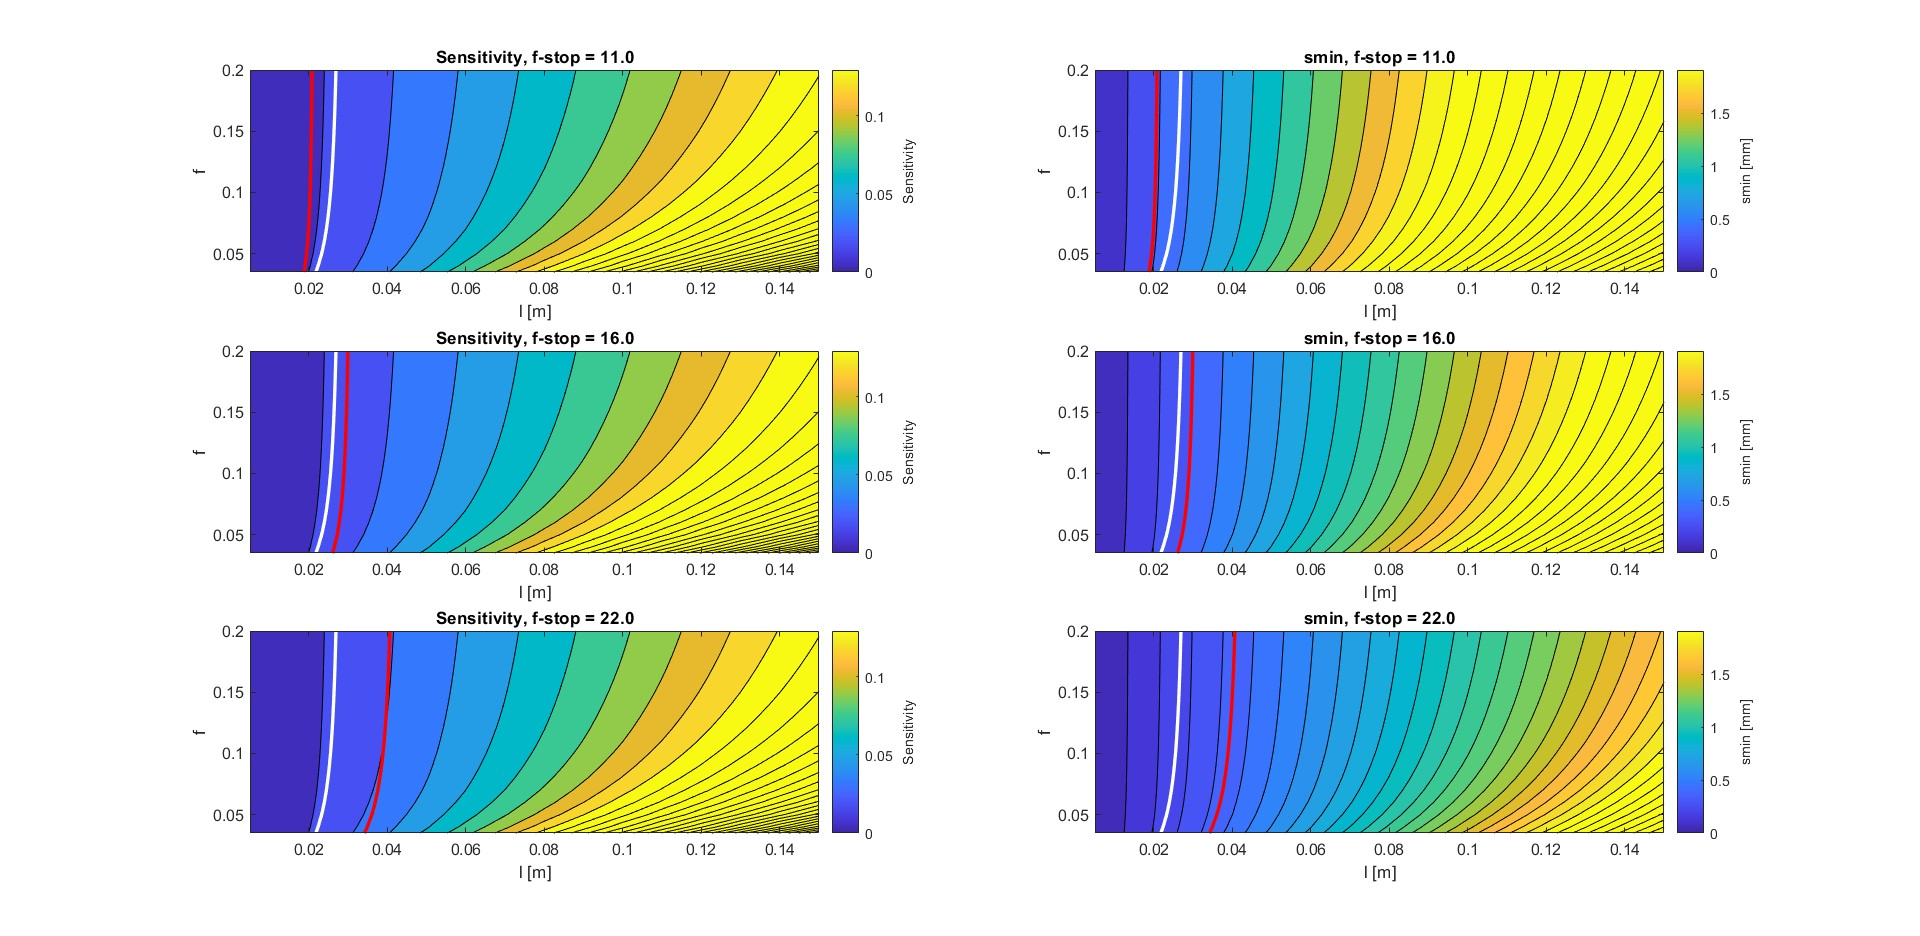
\includegraphics[width=1\textwidth]{figures/Sensitivity and dav SBOS surf map.jpg}
    \caption{Surface maps of $S$ and $s_{min}$ for $f_\# \in $ [11,16,22],  $f \in $ (0.035,0.200) and $l \in$ (0.005,0.15) for a negative defocus setup, with the red isoline representing the points where $s_{min}$ =0.0004 m and the white line showing $S=0.02$.}
    \label{fig: S and dav design surfmap SBOS}
\end{figure}

\par From Figure \ref{fig: S and dav design surfmap SBOS}, it is possible to draw the main trends in the two performance parameters, Sensitivity and $s_{min}$, with changing focal length $f$ and defocus distance $l$. The sensitivity seems to improve with a higher $l$, whereas the spatial resolution is worsened, signaled by an increase in the smallest distinguishable feature size $s_{min}$. For a fixed $l$, both $S$ and $s_{min}$ increase with lower $f$ but the effect becomes less prominent for higher focal length values. This means that a shorter focal length can reach the same sensitivity as a longer one at a smaller $l$, at the cost of a proportionally larger $s_{min}$. Moreover, the larger isoline gaps present at higher $f$ means that the system performance is less prone to changes for small deviations in $l$, which makes it more robust to uncertainties and errors induced during the setup assembly. This means that a higher $f$ and a lower $l$ are desirable for an optimal optical setup.

\par The figure also shows that the f-stop number can be used to easily increase the setup performance, as previously mentioned. When comparing the trends in sensitivity and $s_{min}$ for the 3 different $f_\#$, the red isoline moves more to the right than the white isoline when the f-stop increases. From this, it follows that a higher f-stop allows for better spatial resolution while still maintaining high sensitivity. From equations \ref{equation: df}, \ref{equation: Thin Lens equation}, \ref{equation: M} and \ref{equation: LFoVobj BOS}, it can be seen that $M$, $m$ and $d_f$ are independent of $f_\#$. This means that a change in $f_\#$ can be made by only changing it in the camera lens while maintaining the same optical setup. Consequently, the f-stop should ideally be set to the highest possible to optimize the sensitivity-resolution trade-off.

\par Other important parameters to analyze are the optical magnification $M$ and the distances $m$ and $d_f$, defined in Figure \ref{fig: SBOS with negative l}. The magnification describes how amplified the image is related to the real object and, as previously determined, it influences the sensitivity-resolution. The distances define how close the test section and in-focus plane are from the camera and directly influence $M$, which makes them important practical parameters that define the setup size. Figure \ref{fig: M,m and df design surfmap SBOS} presents the surface maps of these quantities for a given range of P.

\begin{figure}[htbp]
    \centering
    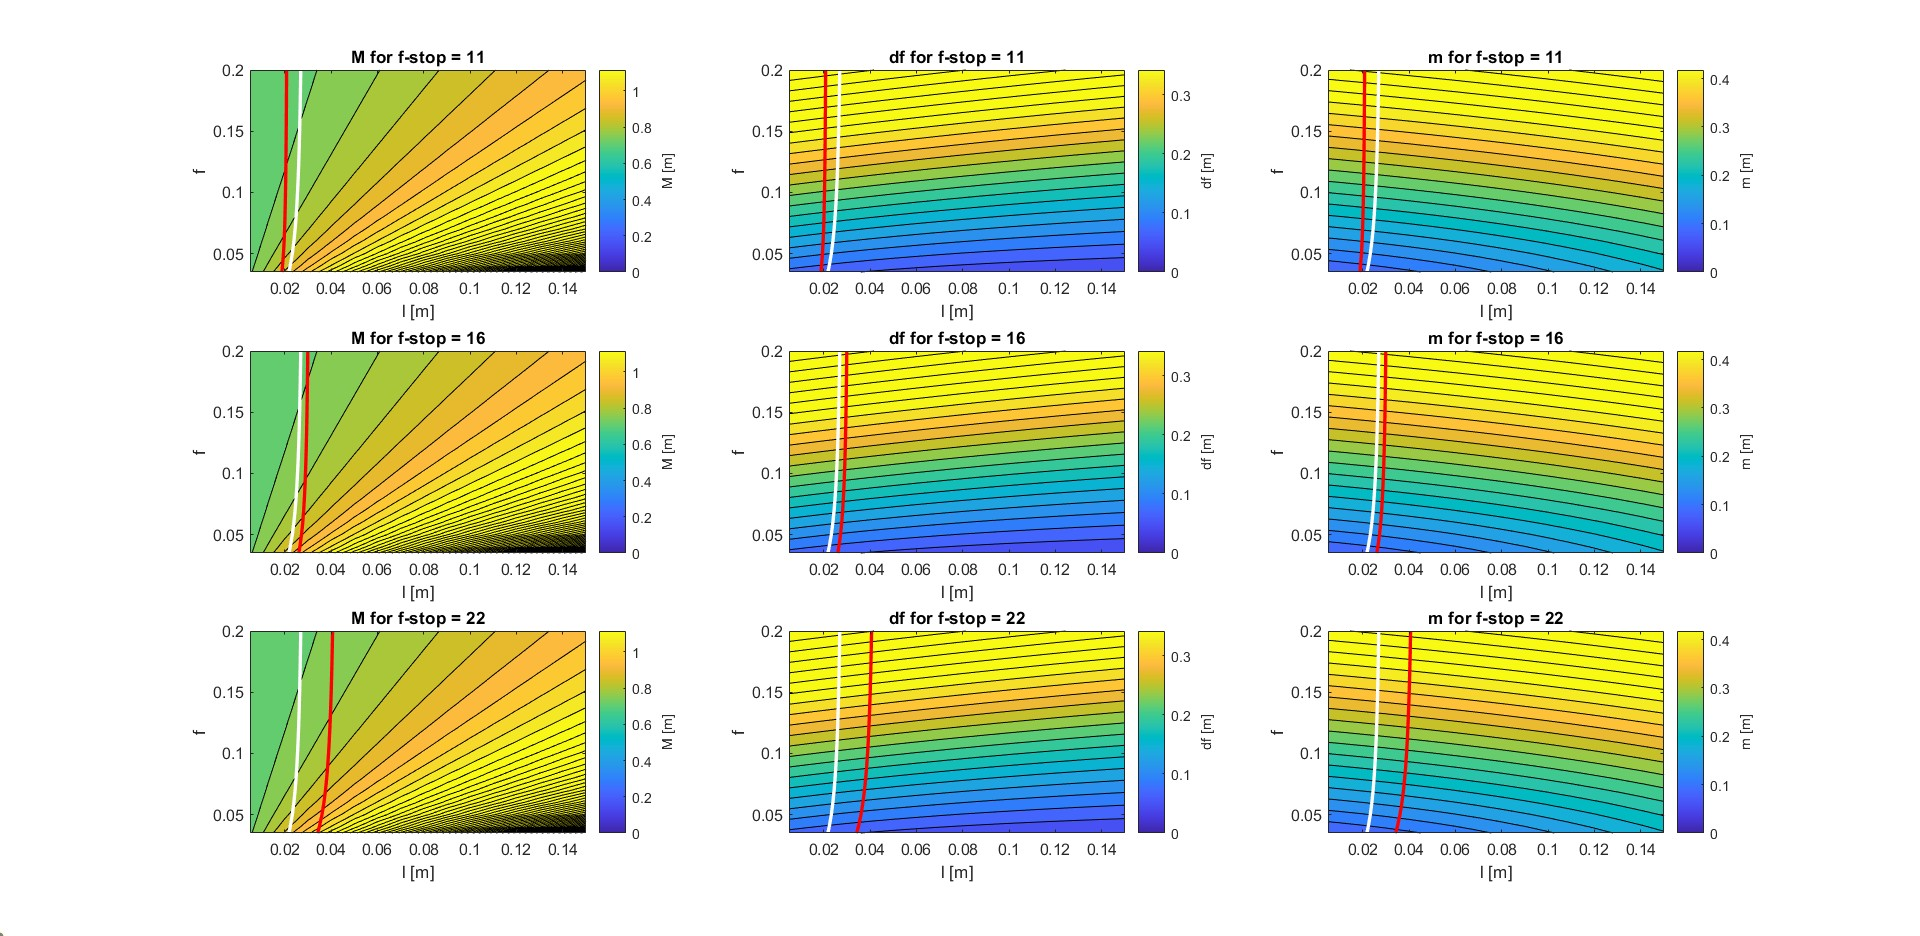
\includegraphics[width=1\textwidth]{figures/M,m,df surfmaps SBOS.jpg}
    \caption{Surface maps of $M$, $m$ and $d_f$ for $f_\# \in $ [11,16,22],  $f \in $ (0.035,0.200), $l \in$ (0.005,0.15) and $L_{FoV_{obj}}=$ 2cm of a negative defocus setup, with the red isoline representing the points where $s_{min}$ =0.0004 m and the white line showing $S=0.02$.}
    \label{fig: M,m and df design surfmap SBOS}
\end{figure}

From Figure \ref{fig: M,m and df design surfmap SBOS}, the distance $m$ only increases slightly along $l$ but presents a steep gradient in the $f$ axis. Together with the findings of Figure \ref{fig: S and dav design surfmap SBOS}, where $S$ and $s_{min}$ don't vary much with $f$, this suggests that a smaller focal length lens could be used to obtain a more compact setup with little cost in sensitivity and spatial resolution. Recall that the gradients of $S$ and $s_{min}$ in relation to $f$ become more intense with lower $f$. Consequently, a moderate focal length such as $f = 0.1$ m is preferable to a considerably shorter one such as $f = 0.05$ m, where the gradients of $S$ and $s_{min}$ are steepest. It can also be argued in favor of $f = 0.1$ m over a longer lens such as $f = 0.2$ m, given the savings in space. Nonetheless, the recommendations made for $f$ earlier in this section still hold, meaning that if the dimension of the setup is not a constraint, a higher $f$ is more desirable.

%\par The Figure also shows the trends on optical magnification. The surface maps show that $M$ increases with higher defocus distance, whereas it tends to decrease with higher$f$. It is true that a higher magnification allows the image to have more pixels per millimeter in the in-focus plane but if the object field of view is fixed, the pixel density in the object plane is also constant. Consequently the ability to capture details of the object is limited to how much blur is present. Figure \ref{fig: S and dav design surfmap SBOS} shows that a smaller $f_\#$ will lead to a blurrier image, so it is possible that a higher magnification won't help increase the resolution. A higher magnification also makes the captured image more prone to errors due to vibrations on the setup. Therefore, a trade-off must be done, where the level of blur is balanced such that the setup resources can be used efficiently. %This paragraph is confusing, I should REVISE it

\par The Figure also shows the trends on optical magnification. The surface maps show that $M$ increases with higher defocus distance, whereas it tends to decrease with higher $f$. The optical magnification can be accurately measured via a calibration plate in the in-focus plane, therefore it will be an important parameter to be validated during the experiment. Moreover, equation \ref{equation: S over smin} shows that the sensitivity-resolution ratio grows monotonically with $M$. 

\par As discussed in chapter \ref{chapter: LiteratureReview}, the minimum speckle size is also an important parameter as it limits the spatial resolution by restricting the allowable interrogation window size on the cross-correlation software. Figure \ref{fig: Delta s design surfmap SBOS} shows how the speckle size changes for a given range of P. Since $\Delta s$ is directly dependent on the magnification through equation \ref{equation: Rayleigh Limit}, it has the same trends as $M$. However, the f-stop number has a much bigger effect in $\Delta s$. It is recommended in the literature to limit the speckle size to 2-5 pixels to ensure optimal cross-correlation and avoid peak locking errors \cite{KahlerEtAl}, which essentially also limits the usable f-stop numbers of the setup. In this studied case, this means that $f_\#$ shouldn't be bigger than 22 nor smaller than 11.

\begin{figure}[htbp]
    \centering
    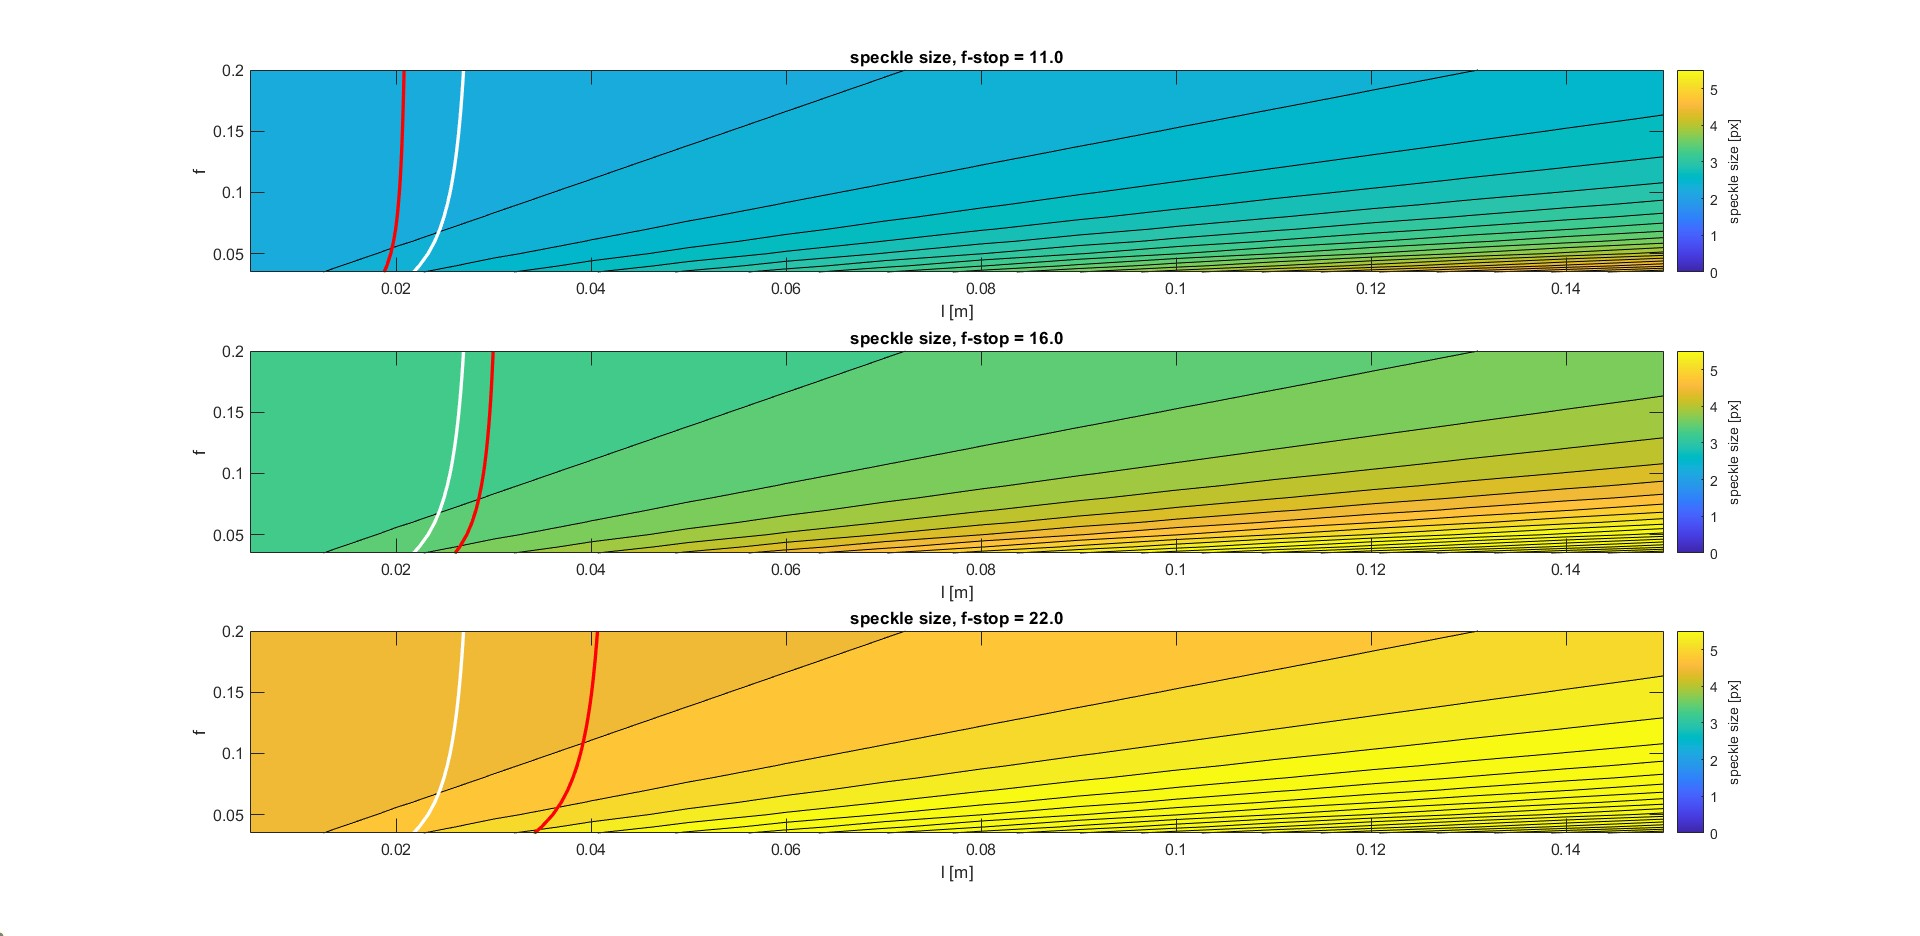
\includegraphics[width=1\textwidth]{figures/Speckle size surf map SBOS.jpg}
    \caption{Surface maps of $\Delta s$ for $f_\# \in $ [11,16,22],  $f \in $ (0.035,0.200), $l \in$ (0.005,0.15) and $L_{FoV_{obj}}=$ 2cm for a negative defocus setup, with the red isoline representing the points where $s_{min}$ =0.0004 m and the white line showing $S=0.02$.}
    \label{fig: Delta s design surfmap SBOS}
\end{figure}

\par It must be said that the speckle generation process is random at its heart \cite{Cloud2007}. The minimum speckle size is defined by the Rayleigh criterion but the average dimension might be bigger than the expected. If it happens that the average speckle size is bigger than 5 pixels, the downside will be the need to use larger interrogation windows, therefore reducing the spatial resolution. Nevertheless, if a high magnification is being used, a big interrogation window might still lead to a small vector pitch and an acceptable resolution. Therefore, there is more to the spatial resolution than the amount of blur in the image as it can also be affected by the CC post-processing. This amounts to the question: how is it possible to reconcile both resolutions such that no resource is being wasted to get a better optical resolution and obtaining a worse processing resolution? Section \ref{section: SR criteria} answers this question and provides a design criterion to choose the best BOS setup. Before getting into the SR criterion, it is worth first analysing how negative defocus compares with positive defocus in the next section.
 
\subsection{Surface Maps for positive defocus setup}
\label{subsection: Surface maps for BOS}

\par Surface maps for a standard BOS setup were also obtained. These maps allow for a comparison of the trends permeating the design space of a positive defocus to the negative defocus present in the last section. Similarly to subsection \ref{subsection: Surface Maps for SBOS}, this subsection will show and discuss the main trends in sensitivity, spatial resolution, $M, m, d_f$ and speckle size $\Delta s$, given $L_{FoV_{obj}}=$ 2cm, $\lambda = 632.8$nm, pixel size equal 6.5 $\mu$m, sensor dimension of 2560x2160 pixels, resulting in $L_{sens}$ = 1.4cm. Figure \ref{fig: S and smin surfmap BOS} contains surface maps of Sensitivity and $s_{min}$ given a range of P.

\begin{figure}[htbp]
    \centering
    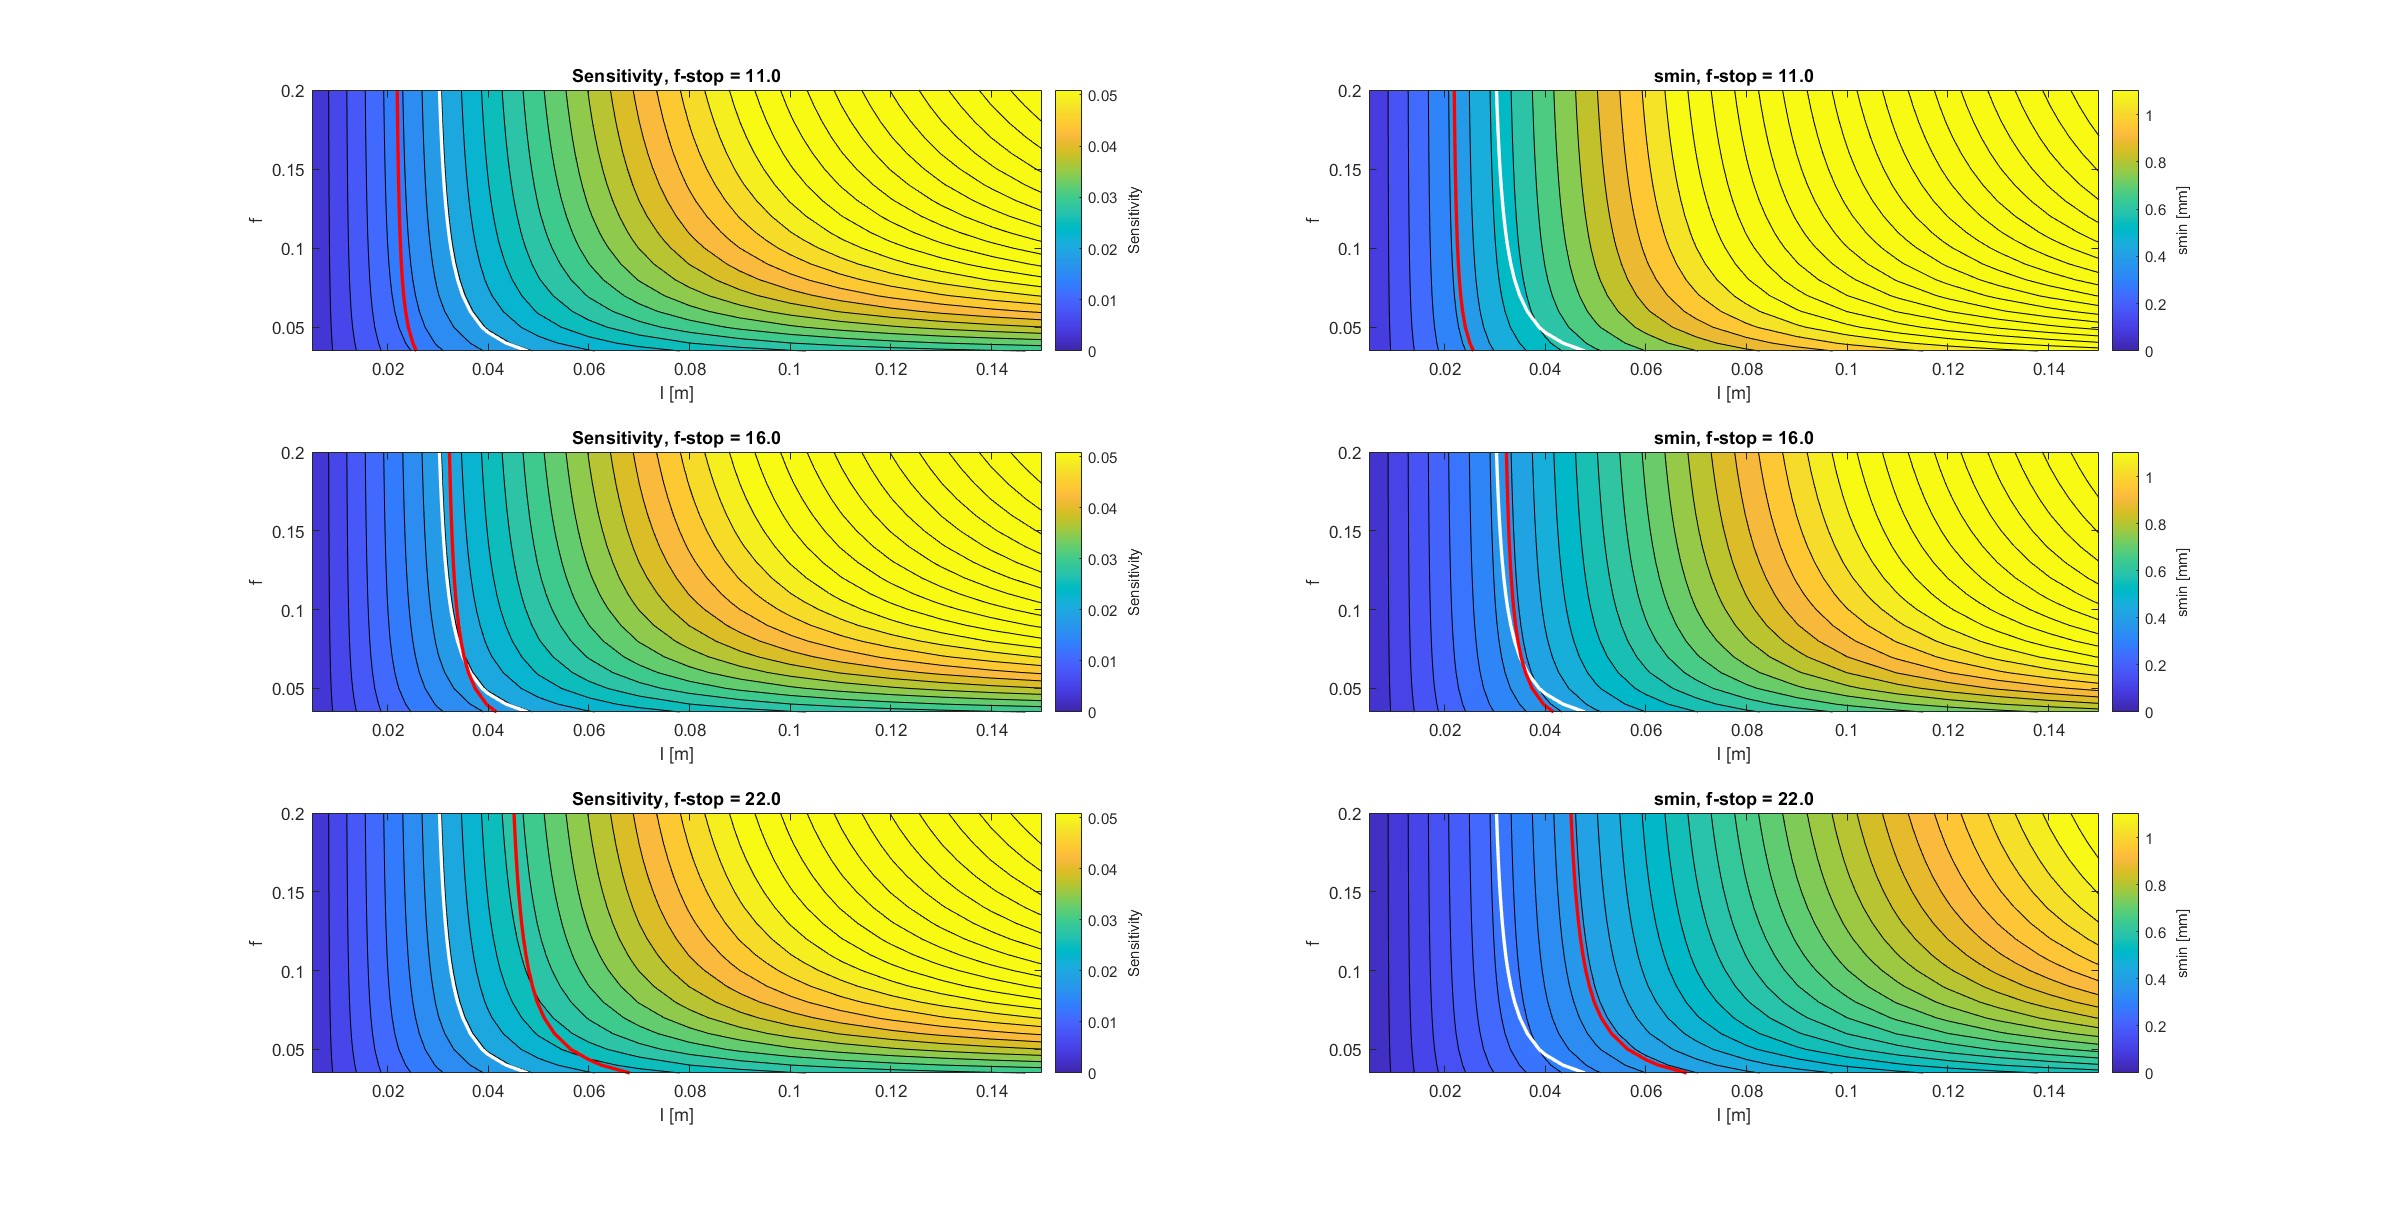
\includegraphics[width=1\textwidth]{figures/Sensitivity and smin BOS surf map.jpg}
    \caption{Surface maps of $S$ and $s_{min}$ for $f_\# \in $ [11,16,22],  $f \in $ (0.035,0.200), $l \in$ (0.005,0.15) and $L_{FoV_{obj}}=$ 2cm of a positive defocus setup, with the red isoline representing the points where $s_{min}$ =0.0004 m and the white line showing $S=0.02$.}
    \label{fig: S and smin surfmap BOS}
\end{figure}

\par Through Figure \ref{fig: S and smin surfmap BOS}, the main trends on sensitivity and spatial resolution for a positive defocus setup can be analyzed. Both parameters seem to reach an asymptote for higher $l$. The higher the $f$, the higher the asymptote value. Moreover, it seems that the sensitivity is unaffected by $f_\#$, while the $s_{min}$ asymptotes moves up and right for an increasing f-stop, meaning that a higher f-stop allows for a better spatial resolution for the same sensitivity, as demonstrated by equation \ref{equation: S over smin}. Recall the discussion from section \ref{section: Background Oriented Schlieren} where a fundamental limit of the sensitivity was obtained by taking the limit for $l \to \infty$. This means that the sensitivity asymptotes shown in Figure \ref{fig: S and smin surfmap BOS} will lead to $S$ converging to $f$, which is summarized in equation \ref{equation: BOS Sensitivity limit}. Consequently, no matter how far away the background is positioned in a positive defocus configuration, the sensitivity will ultimately be limited by the focal length of the camera, whereas with the negative defocus, sensitivity is unbounded. Nevertheless, while designing the setup, the same recommendation reached for SBOS also applies for BOS, a higher focal length and f-stop is the most desirable.

\begin{equation}
    \label{equation: BOS Sensitivity limit}
    \lim_{l \to \infty}S = f
\end{equation}

Regarding $M,m$ and $d_f$, Figure \ref{fig: M,m and df design surfmap BOS} shows that the positive defocus setup variables have different trends compared to a negative one. Variables $m$ and $d_f$ seem to have switched behaviors if compared to their trends in section \ref{subsection: Surface Maps for SBOS}, with $m$ increasing slightly with $l$, while $d_f$ decreases little with $l$, and both increasing considerably with $f$. Due to the large gradient of both distances in the $f$ axis and the nature of the $S$ and $s_{min}$, similarly to the negative defocus case, it is possible to obtain a more compact setup using a smaller focal length if needed, with little loss in sensitivity and spatial resolution. Comparing $M$ from positive $l$ to negative $l$, it is worth noting that the absolute values are smaller and the trend is inverted, which strengthens the argument that SBOS presents a higher $S$ for the same $s_{min}$ due to an increase in $M$. The decrease in $M$ also reflects in a smaller speckle size for the BOS case through equation \ref{equation: Rayleigh Limit}, this can be seen in Appendix \ref{Appendix: Speckle size BOS map}.

\begin{figure}[htbp]
    \centering
    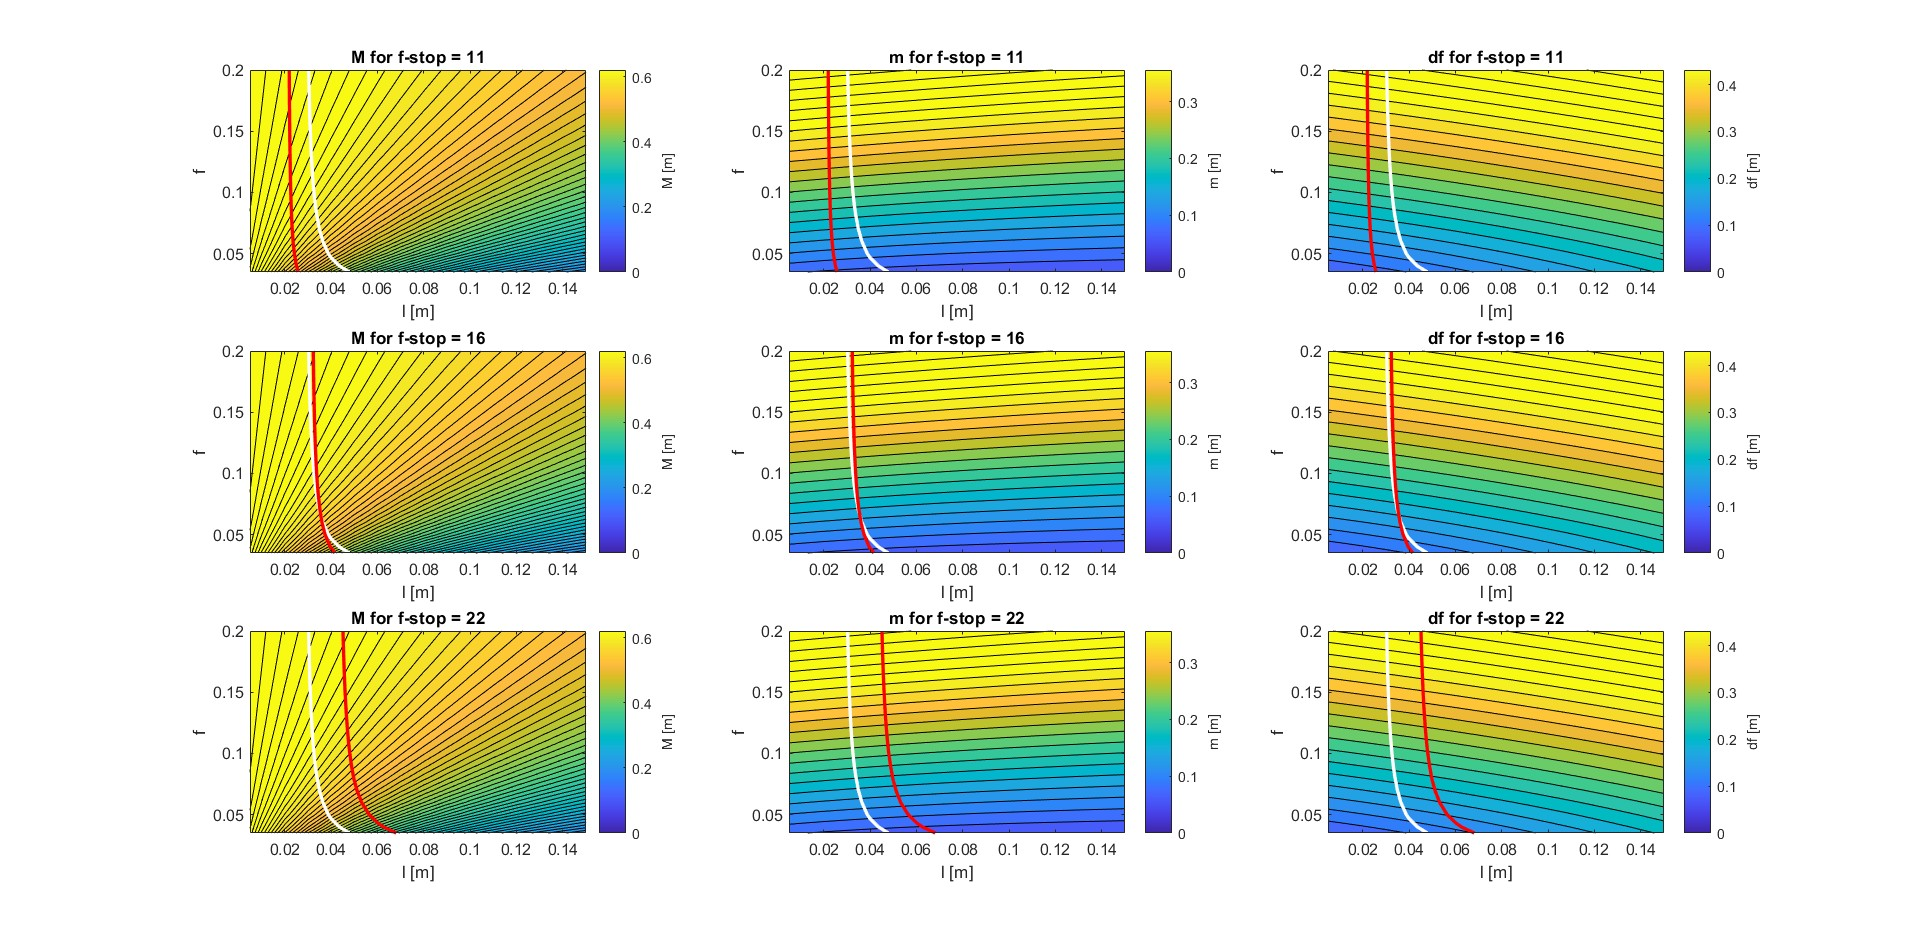
\includegraphics[width=1\textwidth]{figures/M,m,df surfmaps BOS.jpg}
    \caption{Surface maps of $M$, $m$ and $d_f$ for $f_\# \in $ [11,16,22],  $f \in $ (0.035,0.200), $l \in$ (0.005,0.15) and $L_{FoV_{obj}}=$ 2cm of a positive defocus setup, with the red isoline representing the points where $s_{min}$ =0.0004 m and the white line showing $S=0.02$.}
    \label{fig: M,m and df design surfmap BOS}
\end{figure}

\subsection{Effect of FoV}
\label{subsection: Effets of FoV}
\par Since the final goal of this thesis is to implement the SBOS method to a wind-tunnel application, it is also worth investigating the effect of altering the size of the field of view. Surface maps will be used to compare the trends in sensitivity and spatial resolution of negative and positive defocus setups when the $L_{FoV_{obj}}$ is changed from 2cm to 7cm. Figure \ref{fig: Surface maps altering FoV} shows these graphs, surface maps for other parameters can be found in Appendix \ref{Appendix: FoV 70mm maps}. For this case, the red isoline value has been slightly modified to $s_{min}$ =0.00035 m. However it still allows the comparison with previous images given the very small difference between them.

\begin{figure}[htbp]
  \centering
  \begin{subfigure}{0.9\textwidth}
    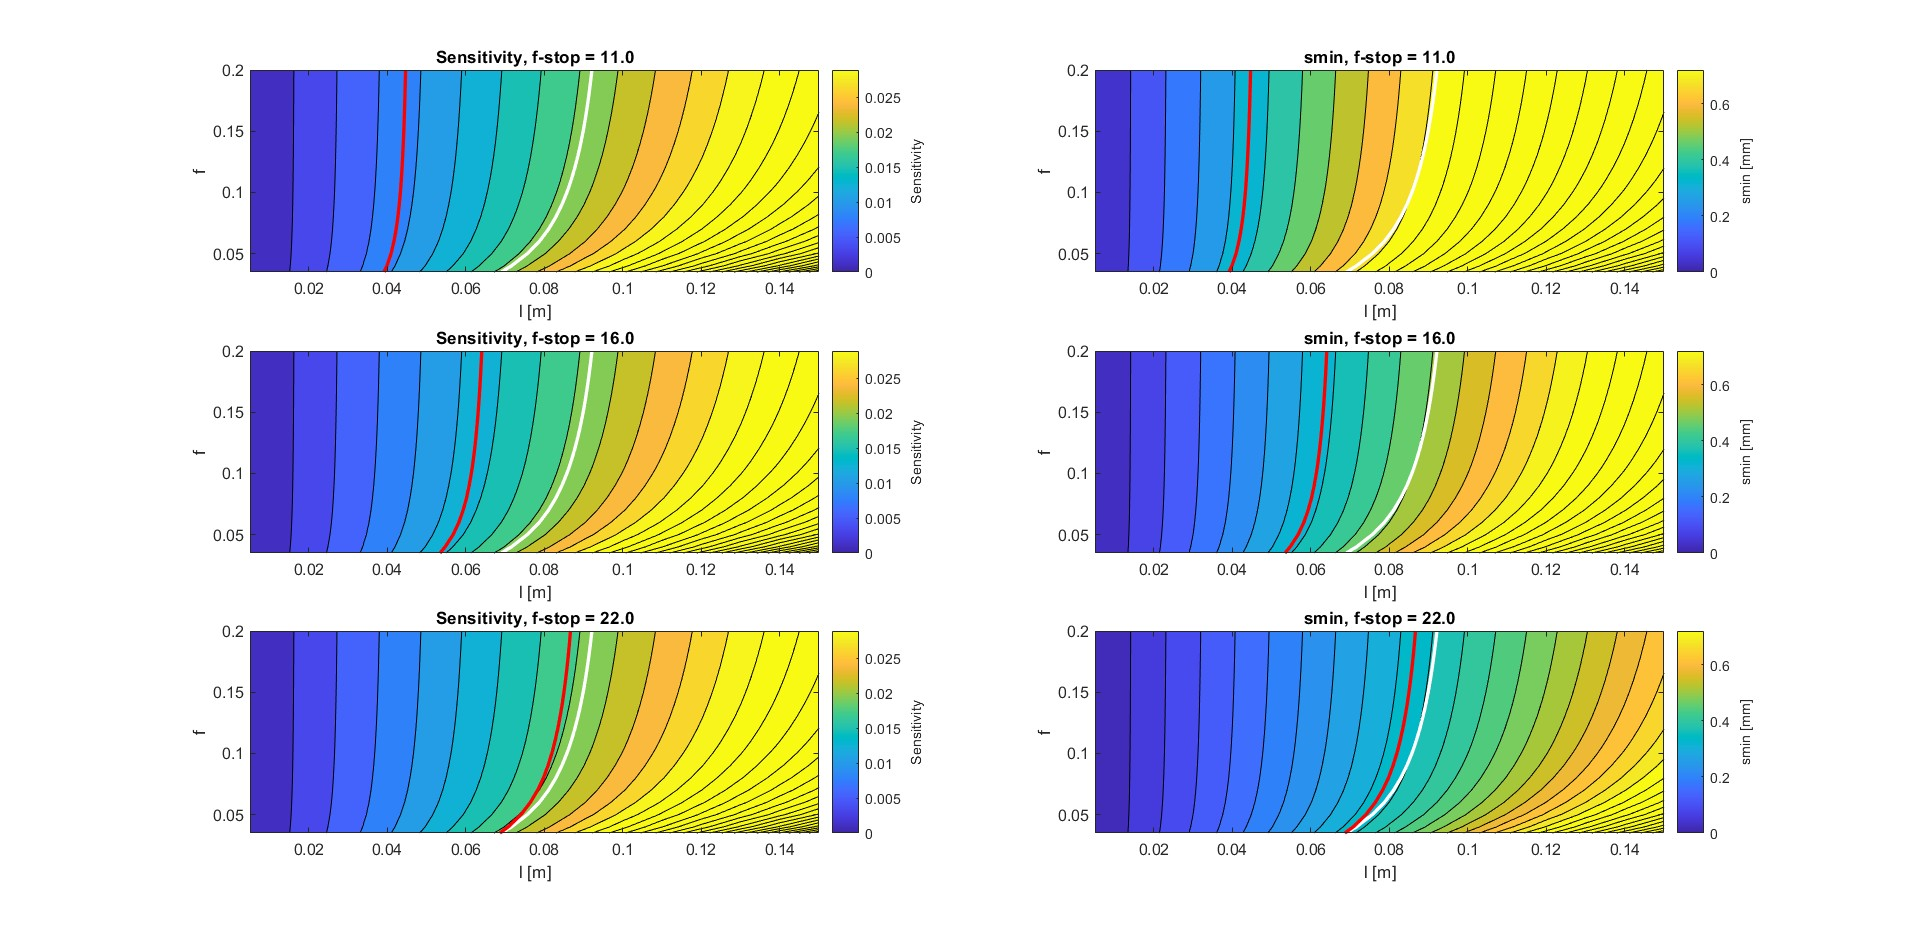
\includegraphics[width=\textwidth]{figures/Sensitivity and smin SBOS surf map 70cm.jpg}
    \caption{}
  \end{subfigure}
  \hfill
  \begin{subfigure}{0.9\textwidth}
    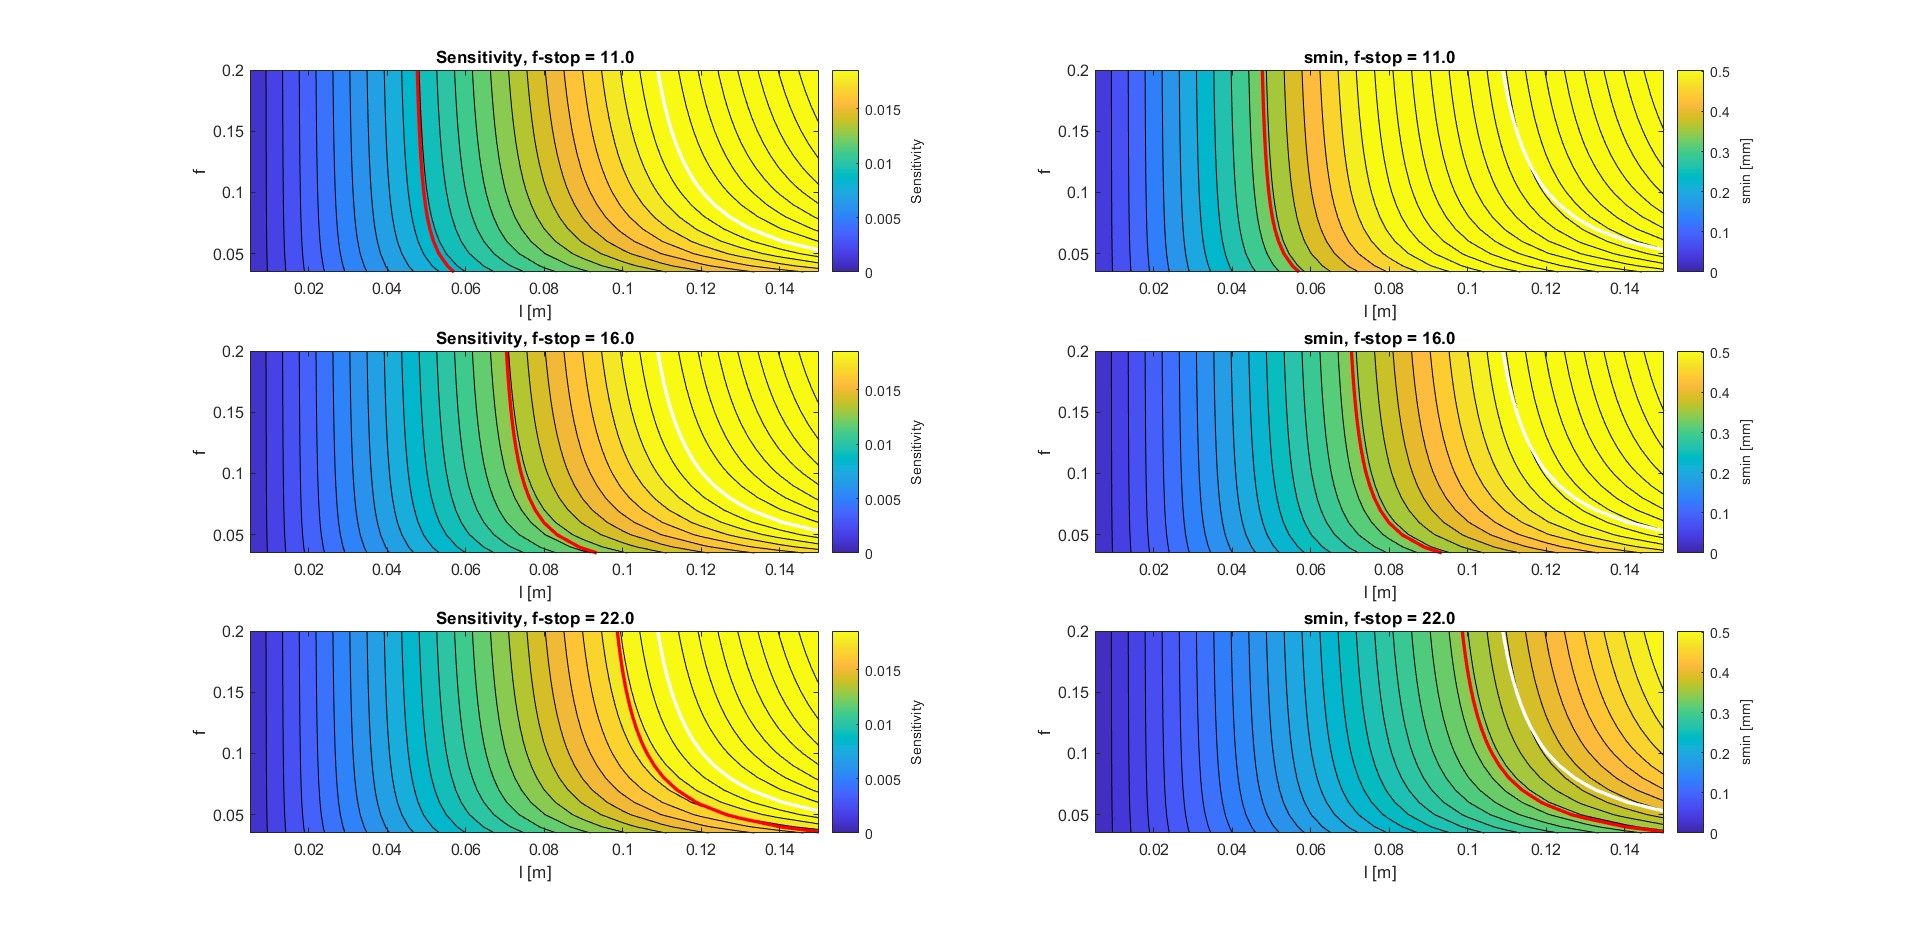
\includegraphics[width=\textwidth]{figures/Sensitivity and smin BOS surf map 70mm.jpg}
    \caption{}
  \end{subfigure}
  \caption{Surface maps of $S$ and $s_{min}$ for $f_\# \in $ [11,16,22],  $f \in $ (0.035,0.200), $l \in$ (0.005,0.15) and $L_{FoV_{obj}}=$ 7cm of a negative defocus setup (a) and a positive defocus setup (b), with the red isoline representing the points where $s_{min}$ =0.00035 m and the white line showing $S=0.02$.}
  \label{fig: Surface maps altering FoV}
\end{figure}

\par From Figure \ref{fig: Surface maps altering FoV} some differences from the surface maps presented at subsections \ref{subsection: Surface Maps for SBOS} and \ref{subsection: Surface maps for BOS} can be highlighted. Generally, a higher field of view results in smaller $S$ and $s_{min}$ due to the smaller optical magnifications needed to achieve the desirable window size, as per equation \ref{equation: M} and \ref{equation: S over smin}. This results in a much higher defocus distance needed to achieve the same $S$. It also translates in less susceptibility to obtain blurred images, which is signaled by the generally smaller $s_{min}$. This is evident from the position of the red and white isolines, which are both located at much higher $l$'s than their smaller $L_{FoV_{obj}}$ counterparts. This characteristic makes the advantage of SBOS even more prominent: with negative defocus a higher sensitivity can be achieved at lower $l$'s while maintaining a low $s_{min}$.

\par Up until now, the surface maps have been useful to visualize the equations displayed in section \ref{section: Geometries of a SBOS optical setup}, \ref{section: Sensitivity-Resolution Ratio} and understand better the trends that exist between variables. However, a definitive criterion to choose the best optical setup is still missing. This will be done by solving a problem mentioned in subsection \ref{subsection: Surface maps for BOS}, to match the optical spatial resolution and software spatial resolution so the experimenter can more efficiently use the its resources. The solution is presented in the next section.

\section{SR criterion}
\label{section: SR criteria}

To reconcile the optical spatial resolution and the post-processing resolution, it must be expressed in terms of pixels. Historically, $M$ has been used by researchers to provide an insight on how much detail the camera can capture, as it defines the pixel density through equation \ref{equation: Px density} \cite{Schmidt2025, Gojani&Obayashi}. However, since the object is blurred, it is not necessarily true that a higher pixel density will lead to a better spatial resolution as the number of pixels per millimeter may increase together with the size of the blur, as per equation \ref{equation: CoC BOS}. 

\par Moreover, given that the object is out of focus, its size differs from the one it would have if it were in focus (see appendix \ref{Appendix: Blurred Object}). Therefore, there are two magnifications at play in the setup, one for the blurred object and another for the in-focus plane. The blurred object magnification is fixed by the desired field of view and camera, defined by equation \ref{equation: M obj}. Whereas the optical magnification shown in Figure \ref{fig: M,m and df design surfmap SBOS} is defined by equation \ref{equation: M}. The amount of detail truly captured by the camera is constrained by $M_{obj}$, fixed by the defined object field of view. It also defines how many pixels can image a mm of the object, through the pixel density (equation \ref{equation: Px density}) and influences the blur of the image, via equation \ref{equation: smin}. Consequently, a trade-off must be done, where the level of blur is balanced with the pixel density such that the setup resources can be used efficiently.

\begin{equation}
    \label{equation: Px density}
    Px_{density} = \frac{M}{Px_{Size}},
    \qquad
    Px_{density_{obj}} = \frac{M_{obj}}{Px_{Size}}
\end{equation}

One way to make this trade-off is to express $s_{min}$ in pixels via Eq. \ref{equation: smin px}, which combines the pixel density with the spatial blur. Dividing the sensor dimension by this quantity gives the ratio $SR$ (Eq. \ref{equation: SR}), which is equivalent to $L_{FoV_{obj}}/s_{min}$ and therefore represents the number of resolvable features across the object field of view. Specifying $SR$ thus fixes how finely the flow is sampled, and with it the number of pixels available to image each feature. For example, $s_{min[px]} = 10$ px ($SR \approx 200$) could be selected: the feature is then spanned by 2–3 speckles and correlated with a 32 px interrogation window at 75\% overlap, giving a vector spacing of 8 px and ensuring the feature is resolved by the vector field.

\begin{equation}
    \label{equation: smin px}
    s_{min_{[px]}} = s_{min} \cdot Px_{density_{obj}}
\end{equation}

\begin{equation}
    \label{equation: SR}
    SR = \frac{L_{sens}}{s_{min_{[px]}} \cdot Px_{Size}}
\end{equation}

\par By defining $SR$, an isoline can be drawn in the surface maps where that condition is met. Together with the previous recommendations: select the highest $f$ for robustness, highest $f_\#$ to obtain the better $S/s_{min}$ trade-off, while keeping $\Delta s$ small enough; the physical distances $l$, $m$ and $d_f$ can be defined. This way, a design point can be selected that optimizes the performance parameters given the available resources.

\section{Summary of Practical Guidelines}
\label{section: Summary of Practical Guidelines}

\par Taken together, the geometric analysis of section \ref{section: Geometries of a SBOS optical setup}, the discussion of section \ref{section: Sensitivity-Resolution Ratio}, the design space exploration of section \ref{section: Design Strategy} and the SR design criterion of section \ref{section: SR criteria} establish a consistent set of guidelines for both BOS and SBOS setups: 

\begin{itemize}
    \item Higher focal length makes the SBOS system more robust to position errors and increases the sensitivity limit for BOS. If size is a constraint, a lower $f$ can result in a more compact setup
    \item A higher f-stop number is generally desirable, subject to the speckle-size constraint of 2–5 pixels
    \item Negative defocus configuration favors a lower defocus distance to exploit its inherent sensitivity advantage over standard BOS
    \item If $f$ and $f_\#$ are maximized, the $SR$ criterion can be used to select the setup that gives the best balance between the optical and CC spatial resolution
    \item SBOS allows for finer speckle sizes than printed BOS, making it possible to study smaller fields of view.
\end{itemize}

Taken together, these guidelines constitute the answer to the first research sub-question posed in Chapter \ref{chapter: introduction}, namely what the practical guidelines for the design of a SBOS setup should be when balancing the trade-off between sensitivity and spatial resolution. They were used to select the design point of the first experimental campaign, balancing sensitivity and spatial resolution. The following chapter describes the resulting experimental setups, built as a proof of concept to validate this design strategy before the method is applied to the more demanding wind tunnel environment. 
